% =============================================================================
%  RESULTS SECTION — revised draft
%  Generated 2026-07-30 against tables/*.tex, figures/*.csv and the code as
%  actually implemented (additional_analysis.py, additional_figures.py,
%  experiments/vss_evpi.py, runner_dispatch._apply_diesel_mode).
%
%  Conventions used below:
%    - plain text   = number confirmed against a stored result file
%    - \red{...}    = still pending a run, or a decision for the authors
% =============================================================================

\subsection{Base-case comparison}
\label{sec:basecase}

Each instance class is instantiated with up to 50 independent random
realizations, and every realization is solved by all five methods (Greedy, RO,
ROBU, LA, SP) and evaluated in the common discrete-event simulator of
Section~\ref{sec:simulation} against the perfect-hindsight oracle.  Coverage is
not uniform: the short and medium route classes are complete at 50 seeds for
Greedy, RO, LA and SP, whereas ROBU terminates within its wall-clock budget
only on the short routes, and on the long routes only Greedy is complete
(RO and LA reach 6--9 seeds per class, SP none).  The per-cell counts in
Table~\ref{tab:gap} make this explicit, and the figures draw the full
canonical grid with the missing slots left empty rather than silently
dropping them.  We compare the methods along three axes.  First, efficiency,
shown through the gap to oracle in realized route duration in
Table~\ref{tab:gap} and Figure~\ref{fig:resultsgap}.  Then, reliability, via
the rate at which the executed schedule becomes infeasible (the infeasibility
strip of Figure~\ref{fig:resultsgap} and Table~\ref{tab:feasibility}).
Finally, computational effort in Table~\ref{tab:runtime}.

Because the oracle is itself a mixed-integer program, the reference against
which every gap is measured is only as tight as its own certificate.
Figure~\ref{fig:boundsoracle} reports, per route class, the incumbent and the
best dual bound of the oracle solves.  On short and medium routes the oracle
closes to within \red{XX\%}; on the long routes the incumbent stabilises early
while the dual bound stalls at roughly 9\%, a structural weakness of the
formulation (the fifth packing-forced rest is not implied by the aggregate
resource constraints) rather than a search failure.  Long-route gaps in
Table~\ref{tab:gap} should therefore be read as ``certified to within
$\approx$9\%'' and not as exact distances to the optimum.

\begin{table}[htbp]
\centering
\caption{Gap to oracle (\%) in route duration (window penalties included) by instance class and method, averaged over 2--50 seed(s) per instance class; travel-time multiplier $\xi_i$ shifted-lognormal on $[0.889, 1.6]$ with $\mathrm{E}[\xi]=1$, $\mathrm{CV} = 0.15$.  Parentheses give the feasible/total run count per cell among runs the oracle bound can assess (a single number when all were feasible); square brackets give feasible runs still awaiting an oracle bound, which are excluded from both counts.  LA uses 25 scenarios over a 24\,h horizon; SP uses 25 scenarios.}
\label{tab:gap}
\begin{tabular}{lll c ccccc}
\toprule
\multirow{2}{*}{\textbf{\small Route}} & \multirow{2}{*}{\textbf{\small Cust.}} & \multirow{2}{*}{\textbf{\small TW}} & \multirow{2}{*}{\textbf{Oracle (h)}} &
\multicolumn{5}{c}{\textbf{Gap to Oracle \%}} \\
\cmidrule(lr){5-9}
 & & & & Greedy & RO & ROBU & LA & SP \\
\midrule
\multirow{12}{*}{\small Short} & \multirow{4}{*}{\small Few} & {\small None} & 26.2 & 12.5~{\scriptsize(40)} & 22.7~{\scriptsize(50)} & 15.3~{\scriptsize(48/50)} & 7.9~{\scriptsize(48/50)} & 4.7~{\scriptsize(48/50)} \\
 &  & {\small Tight} & 25.9 & 19.1~{\scriptsize(39/40)} & 28.4~{\scriptsize(50)} & 16.9~{\scriptsize(50)} & 11.3~{\scriptsize(50)} & 5.0~{\scriptsize(44/50)} \\
 &  & {\small Medium} & 26.1 & 17.3~{\scriptsize(39/40)} & 25.0~{\scriptsize(50)} & 17.4~{\scriptsize(48/50)} & 11.3~{\scriptsize(50)} & 5.0~{\scriptsize(45/50)} \\
 &  & {\small Large} & 25.9 & 16.3~{\scriptsize(40)} & 23.4~{\scriptsize(50)} & 15.1~{\scriptsize(46/49)} & 10.0~{\scriptsize(50)} & 5.0~{\scriptsize(46/50)} \\
 & \multirow{4}{*}{\small Medium} & {\small None} & 28.0 & 12.7~{\scriptsize(50)} & 20.9~{\scriptsize(50)} & 16.1~{\scriptsize(49/50)} & 8.8~{\scriptsize(50)} & 4.3~{\scriptsize(46/50)} \\
 &  & {\small Tight} & 28.0 & 28.3~{\scriptsize(49/50)} & 36.9~{\scriptsize(50)} & 27.7~{\scriptsize(48/50)} & 15.2~{\scriptsize(50)} & 5.7~{\scriptsize(46/50)} \\
 &  & {\small Medium} & 27.6 & 22.1~{\scriptsize(49/50)} & 30.6~{\scriptsize(50)} & 19.0~{\scriptsize(50)} & 11.6~{\scriptsize(49)} & 4.6~{\scriptsize(45/50)} \\
 &  & {\small Large} & 28.2 & 17.2~{\scriptsize(49/50)} & 34.0~{\scriptsize(50)} & 24.2~{\scriptsize(48/50)} & 11.5~{\scriptsize(50)} & 3.6~{\scriptsize(46/50)} \\
 & \multirow{4}{*}{\small Many} & {\small None} & 31.0 & 15.2~{\scriptsize(40)} & 28.0~{\scriptsize(50)} & 23.2~{\scriptsize(49/50)} & 6.8~{\scriptsize(50)} & 5.6~{\scriptsize(49/50)} \\
 &  & {\small Tight} & 31.1 & 42.8~{\scriptsize(40)} & 53.4~{\scriptsize(50)} & 47.1~{\scriptsize(47/49)} & 17.9~{\scriptsize(47/50)} & 11.4~{\scriptsize(44/50)} \\
 &  & {\small Medium} & 31.5 & 32.6~{\scriptsize(39/40)} & 49.3~{\scriptsize(50)} & 37.6~{\scriptsize(48/49)} & 23.1~{\scriptsize(49/50)} & 6.2~{\scriptsize(45/50)} \\
 &  & {\small Large} & 30.2 & 19.0~{\scriptsize(40)} & 40.2~{\scriptsize(50)} & 25.2~{\scriptsize(46/50)} & 12.8~{\scriptsize(50)} & 4.8~{\scriptsize(46/50)} \\
\midrule
\multirow{12}{*}{\small Medium} & \multirow{4}{*}{\small Few} & {\small None} & 53.8 & 16.5~{\scriptsize(38/40)} & 38.6~{\scriptsize(50)} & -- & 11.8~{\scriptsize(47/50)} & 13.7~{\scriptsize(42/50)} \\
 &  & {\small Tight} & 55.3 & 18.2~{\scriptsize(40)} & 35.2~{\scriptsize(50)} & -- & 11.2~{\scriptsize(49/50)} & 12.3~{\scriptsize(44/50)} \\
 &  & {\small Medium} & 53.5 & 16.5~{\scriptsize(40)} & 37.7~{\scriptsize(50)} & -- & 11.7~{\scriptsize(48/49)} & 9.9~{\scriptsize(46/50)} \\
 &  & {\small Large} & 53.9 & 13.8~{\scriptsize(38/40)} & 35.8~{\scriptsize(50)} & 60.6~{\scriptsize(1)} & 10.8~{\scriptsize(49/50)} & 9.5~{\scriptsize(42/50)} \\
 & \multirow{4}{*}{\small Medium} & {\small None} & 57.3 & 12.8~{\scriptsize(50)} & 30.1~{\scriptsize(50)} & -- & 8.1~{\scriptsize(49/50)} & 10.2~{\scriptsize(44/50)} \\
 &  & {\small Tight} & 56.2 & 22.0~{\scriptsize(49/50)} & 36.4~{\scriptsize(50)} & -- & 15.0~{\scriptsize(45/46)} & 12.2~{\scriptsize(7/8)} \\
 &  & {\small Medium} & 55.8 & 19.4~{\scriptsize(49/50)} & 38.8~{\scriptsize(50)} & -- & 13.6~{\scriptsize(50)} & 11.9~{\scriptsize(40/50)} \\
 &  & {\small Large} & 55.0 & 16.5~{\scriptsize(50)} & 36.8~{\scriptsize(50)} & -- & 9.9~{\scriptsize(50)} & 10.8~{\scriptsize(41/50)} \\
 & \multirow{4}{*}{\small Many} & {\small None} & 59.3 & 14.5~{\scriptsize(40)} & 29.1~{\scriptsize(50)} & -- & 10.5~{\scriptsize(47/48)} & 11.9~{\scriptsize(43/50)} \\
 &  & {\small Tight} & 59.4 & 32.4~{\scriptsize(40)} & 46.0~{\scriptsize(50)} & -- & 27.0~{\scriptsize(47)} & 27.4~{\scriptsize(40/47)} \\
 &  & {\small Medium} & 59.5 & 28.2~{\scriptsize(40)} & 42.4~{\scriptsize(50)} & -- & 21.0~{\scriptsize(47/48)} & 19.5~{\scriptsize(38/49)} \\
 &  & {\small Large} & 58.1 & 19.9~{\scriptsize(39/40)} & 41.7~{\scriptsize(50)} & -- & 15.3~{\scriptsize(48/50)} & 16.3~{\scriptsize(41/49)} \\
\midrule
\multirow{12}{*}{\small Long} & \multirow{4}{*}{\small Few} & {\small None} & 102.8 & 11.7~{\scriptsize(49/50)} & 33.8~{\scriptsize(9)} & -- & 11.0~{\scriptsize(8)} & -- \\
 &  & {\small Tight} & 105.7 & 14.7~{\scriptsize(26/29)} & 37.8~{\scriptsize(9)} & -- & 9.9~{\scriptsize(9)} & -- \\
 &  & {\small Medium} & 105.5 & 14.2~{\scriptsize(50)} & 35.9~{\scriptsize(9)} & -- & 8.9~{\scriptsize(8)} & -- \\
 &  & {\small Large} & 105.0 & 12.3~{\scriptsize(44/46)} & 37.0~{\scriptsize(9)} & -- & 9.2~{\scriptsize(9)} & -- \\
 & \multirow{4}{*}{\small Medium} & {\small None} & 104.8 & 11.9~{\scriptsize(49/50)} & -- & -- & 8.5~{\scriptsize(6)} & -- \\
 &  & {\small Tight} & 104.4 & 18.1~{\scriptsize(14/15)} & -- & -- & 11.6~{\scriptsize(6/7)} & -- \\
 &  & {\small Medium} & 105.6 & 15.3~{\scriptsize(49/50)} & 36.0~{\scriptsize(7)} & -- & 11.5~{\scriptsize(7)} & -- \\
 &  & {\small Large} & 104.3 & 14.0~{\scriptsize(49/50)} & 38.6~{\scriptsize(9)} & -- & 10.4~{\scriptsize(8)} & -- \\
 & \multirow{4}{*}{\small Many} & {\small None} & 113.9 & 8.0~{\scriptsize(1/4)[39]} & 34.2~{\scriptsize(1)[8]} & -- & --~{\scriptsize(0/1)[7]} & -- \\
 &  & {\small Tight} & -- & --~{\scriptsize(0/2)[48]} & --~{\scriptsize[9]} & -- & --~{\scriptsize[8]} & -- \\
 &  & {\small Medium} & 107.9 & 25.0~{\scriptsize(2/3)} & 34.5~{\scriptsize(8)[1]} & -- & 11.8~{\scriptsize(7)} & -- \\
 &  & {\small Large} & 109.6 & 13.4~{\scriptsize(23)} & 34.1~{\scriptsize(9)} & -- & 12.8~{\scriptsize(8)} & -- \\
\bottomrule
\end{tabular}
\end{table}

\begin{figure}[htbp]
    \centering
    % \red{PLACEHOLDER} — three panels produced by oracle_bound_multi_optimality.py:
    % figures/oracle_bounds_opt_short.pdf, _medium.pdf, _long.pdf
    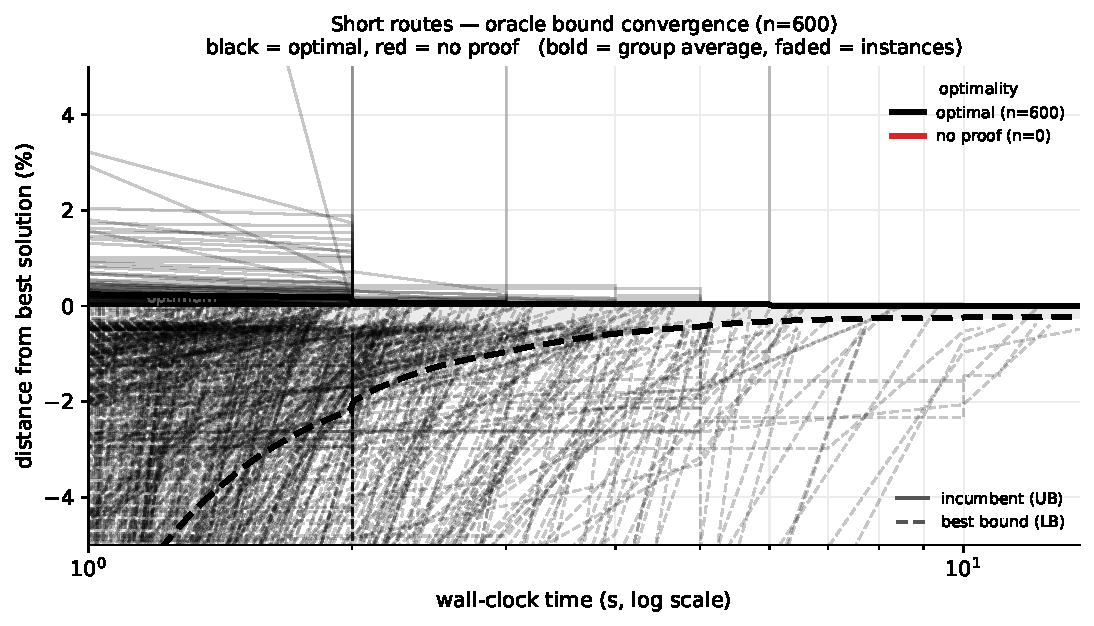
\includegraphics[width=\linewidth]{figures/oracle_bounds_opt_short.pdf}\\[2pt]
    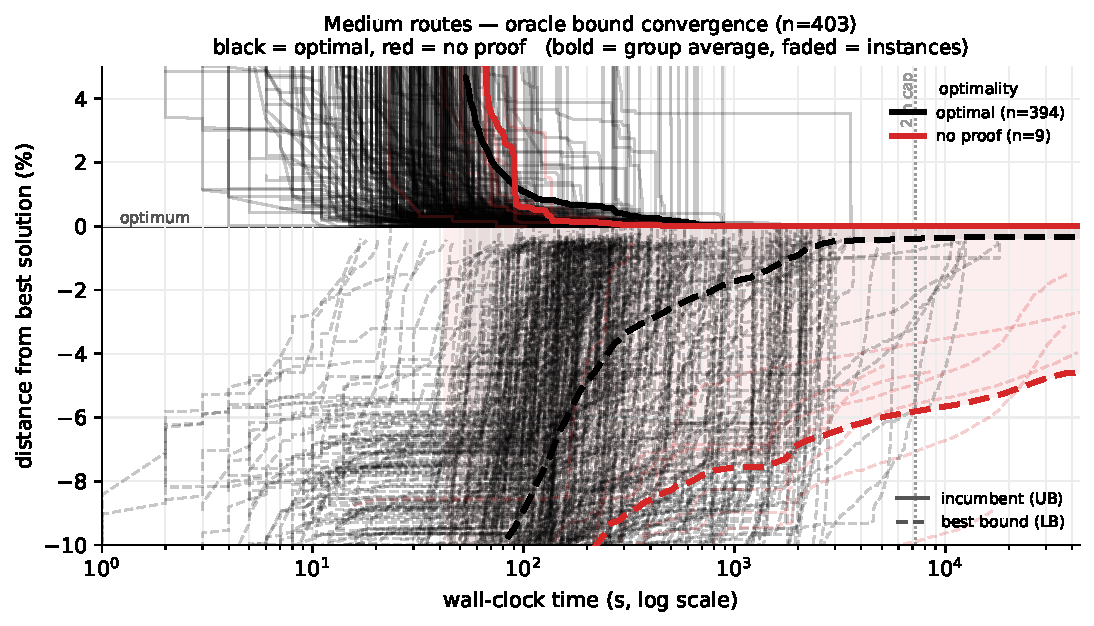
\includegraphics[width=\linewidth]{figures/oracle_bounds_opt_medium.pdf}\\[2pt]
    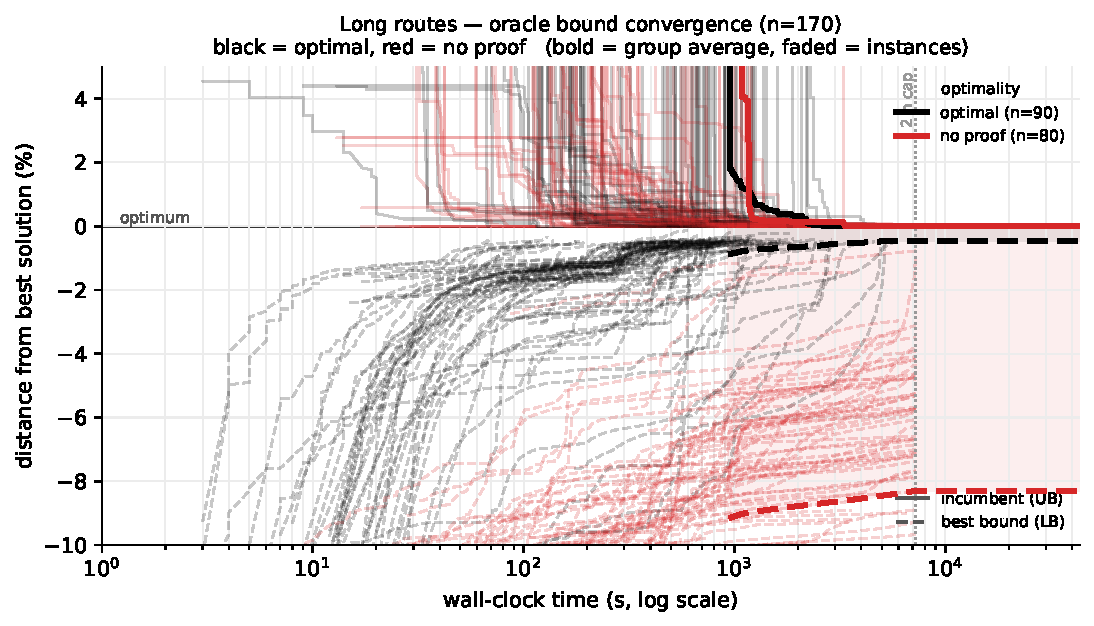
\includegraphics[width=\linewidth]{figures/oracle_bounds_opt_long.pdf}
    \caption{Convergence of the perfect-hindsight oracle by route class:
    incumbent objective (solid) against the best dual bound (dashed) over
    wall-clock time, one trace per instance, 2\,h cap.  Short and medium
    instances close to \red{XX\%}; on long routes the incumbent settles within
    minutes while the dual bound stalls near 9\%, so long-route gaps are
    certified-to-9\% rather than exact.}
    \label{fig:boundsoracle}
\end{figure}

\begin{figure}[htbp]
    \centering
    % \red{PLACEHOLDER} — produced by `python paper_figures.py --all`:
    % figures/paper_gap_box.pdf   (method blocks, each holding its four TW boxes)
    % figures/paper_gap_box_methods.pdf (TW blocks, each holding the four methods)
    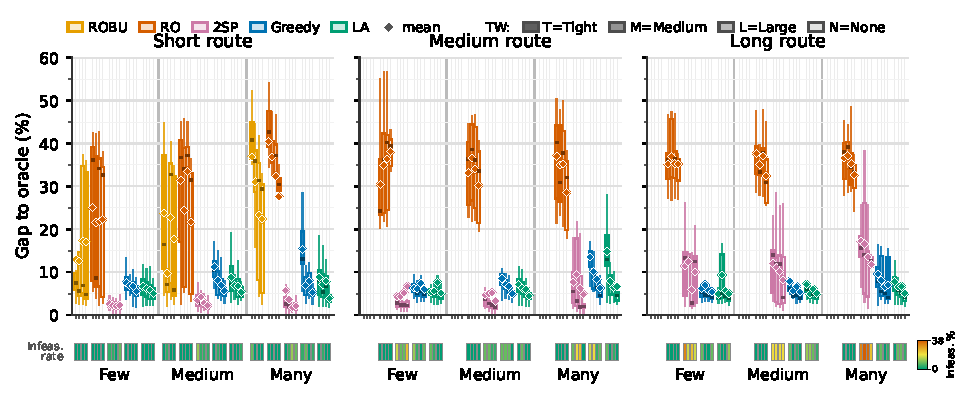
\includegraphics[width=\linewidth]{figures/paper_gap_box.pdf}
    \caption{Distribution of the realized gap to the oracle across seeds, by
    route class (rows), customer count (columns), method (colour) and
    time-window class (shade, Tight--Medium--Large--None).  Boxes span the
    interquartile range, whiskers 1.5\,IQR.  The heat strip below each panel
    shades the \emph{genuine} infeasibility rate --- certified plans that still
    fail in execution --- with a diagonal hatch marking cells that also contain
    uncertified (unsolved) runs, so a non-converged solve is never read as a
    failure.  Empty slots are instance/method combinations without completed
    runs.}
    \label{fig:resultsgap}
\end{figure}

Across instance classes the two-stage stochastic plan (SP) and the look-ahead
policy (LA) attain the smallest gaps to the oracle (SP 3.6--27.4\%, mean
9.6\%; LA 6.8--27.0\%, mean 12.3\%), the myopic greedy heuristic is
intermediate (8.0--42.8\%, mean 18.4\%), and the static robust plans are the
most conservative (ROBU 15.1--60.6\%, mean 26.6\%; RO 20.9--53.4\%, mean
35.3\%).  This ordering follows the amount of information each method uses and
the point at which it commits: the two policies that adapt to realised travel
times---SP through online duration recourse and LA through full
re-optimisation at every stop---recover most of the hindsight optimum, whereas
the offline robust plans pay for committing every duration in advance against a
worst case.  The ordering between SP and LA reverses with route length: on the
short routes SP is clearly ahead (5.5\% vs.\ 12.3\% on average) because 25
scenarios over the whole horizon still capture the realisation well, while on
the medium routes the two are indistinguishable (13.8\% each) and on the long
routes SP no longer terminates at all.  Greedy, conversely, improves in
relative terms as routes lengthen (21.3\%, 19.2\%, 14.4\% mean gap on short,
medium and long routes): on a 100\,h route the mandatory rest structure
dominates and there is little left for a planner to exploit.

The gap widens sharply with the number of customers and the tightness of the
windows.  On the short routes the \emph{Few}/\emph{Large} cell gives
16.3/23.4/15.1/10.0/5.0\% for Greedy/RO/ROBU/LA/SP, against
42.8/53.4/47.1/17.9/11.4\% on \emph{Many}/\emph{Tight}---a two- to
three-fold deterioration for the three committing methods and less than a
doubling for the two adaptive ones.  A static schedule that must satisfy more,
and narrower, service windows simultaneously is exactly the situation in which
committing early is most expensive.

A substantial part of the gap on the window-constrained classes is window
penalty rather than slower routing, but the split runs opposite to what one
might expect.  Comparing the penalised gap of Table~\ref{tab:gap} with the
duration-only gap of Table~\ref{tab:gap-nopen}, the $\beta\sum_i\delta_i$ term
accounts on average for 16\% of RO's gap and 21\% of Greedy's, and on the
tight-window classes for 25\% of RO's (range 4--48\%) against 37\% of
Greedy's (9--66\%).  The penalty share is thus \emph{smallest} for the box
robust plan: RO is genuinely slower, spending its gap on conservative
durations, while Greedy's tight-window gap is mostly the cost of arriving off
the windows---up to two-thirds of it on \emph{Short}/\emph{Many}/\emph{Tight}
(42.8\% penalised vs.\ 14.5\% duration-only).  The adaptive policies sit in
between (LA 38\%, SP 35\% on tight windows), consistent with policies that buy
window compliance with a little extra time.  On the window-free classes the two
gap definitions coincide exactly, as they must.

Where both static robust variants terminate---the twelve short-route
classes---the budgeted plan (ROBU) improves on the box plan (RO) in every
single cell, by 4.8 to 15.0 percentage points (23.7\% vs.\ 32.7\% on average;
e.g.\ 19.0\% vs.\ 30.6\% on \emph{Short}/\emph{Medium}/\emph{Medium}).  This
confirms that pricing only a bounded number of legs at their worst case removes
a large part of the box's conservatism while retaining a guarantee
(Section~\ref{sec:robu}).  \red{The single medium-route ROBU cell
(\emph{Medium}/\emph{Few}/\emph{Large}, 60.6\% on one seed) is a
non-representative outlier from a run that hit its wall-clock budget; either
complete that class or drop the cell before submission.}

\begin{table}[htbp]
\centering
\caption{Feasibility and robustness statistics by method: HoS-violation rate, stranding rate, repair frequency (offline plans), and window hit rate, computed over runs whose plan the solver certified.  ``Not opt.'' is the share of runs returned at the time limit without a proven optimum; ``Not solved'' the share whose plan was never certified (excluded from the rates to their left).}
\label{tab:feasibility}
\begin{tabular}{lcccccc}
\toprule
\textbf{Method} & \textbf{HoS viol. (\%)} & \textbf{Stranding (\%)} & \textbf{Repairs (\%)} & \textbf{TW hit (\%)} & \textbf{Not opt. (\%)} & \textbf{Not solved (\%)}\\
\midrule
Greedy & 2.2 & 0.2 & -- & 55.0 & -- & 0.0 \\
RO & 0.0 & 0.0 & 0.0 & 44.9 & 14.2 & 0.0 \\
ROBU & 0.0 & 3.3 & 0.0 & 67.3 & 8.5 & 6.0 \\
LA (25S-24h) & 0.5 & 1.0 & -- & 69.7 & -- & 0.0 \\
SP (25S) & 0.3 & 11.6 & 99.0 & 86.6 & 36.1 & 0.0 \\
\bottomrule
\end{tabular}
\end{table}

Efficiency alone is misleading, because a favorable gap can hide a high failure
rate: infeasible runs (a stranding or an Hours-of-Service breach in execution)
carry no meaningful gap and are excluded from the averages, so a method that
fails often is scored only on the realizations it survives.  The infeasibility
strip of Figure~\ref{fig:resultsgap} and Table~\ref{tab:feasibility} restore
this axis.  Two failure modes must be kept apart, and the table separates them:
a \emph{genuine} infeasibility, where the solver certified a plan and execution
still broke it, and an \emph{unsolved} run, where no plan was ever certified.
Only ROBU has a non-zero unsolved share (6.0\%), and those runs are excluded
from the rates to their left rather than counted as failures.

The two-stage plan attains the best window compliance in the study
(TW hit 86.6\%) and among the lowest gaps, but only through near-permanent
online recourse: it repairs its committed structure on 99.0\% of runs and still
strands the vehicle on 11.6\%---by an order of magnitude the highest stranding
rate of the five methods.  A plan that must be repaired on essentially every
execution is, in practice, a policy rather than a plan, and the 36.1\% of SP
solves returned at the time limit without a proven optimum reinforces that
reading.  The robust plans never breach the Hours-of-Service rules by
construction, and RO never strands either, at the cost of the worst window
compliance (44.9\%) and the largest gaps; ROBU trades a 3.3\% stranding rate
for a 22-point gain in window hit rate (67.3\%) and a 9-point gain in gap.
\red{The ROBU strandings deserve a sentence of diagnosis: since the budget
$\Gamma$ is applied to the time uncertainty while the energy corner is priced
at $\xi_{\min}$, a realisation that is simultaneously fast (high ECR) on more
than $\Gamma$ legs is outside the protected set. Confirm against the
$\Gamma$-frontier runs of Section~\ref{sec:uncertainty} before writing it as
fact.}  The greedy heuristic rarely strands (0.2\%) but breaches driving limits
on 2.2\% of runs---the only method with a material HoS violation rate---and
misses the most windows after RO (TW hit 55.0\%), consistent with a policy that
stops only when forced.  The look-ahead policy is the only method that is
simultaneously highly feasible (0.5\% HoS, 1.0\% stranding) and
window-compliant (69.7\%) without any recourse machinery, which is what makes
it the most defensible operational recommendation even though SP dominates it
on the short routes.

\begin{table}[htbp]
\centering
\caption{Computation times by method and instance class: offline solve time (s) and per-stop online decision time (s).}
\label{tab:runtime}
\begin{tabular}{lcccccc}
\toprule
& \multicolumn{3}{c}{\textbf{Offline solve (s)}} & \multicolumn{3}{c}{\textbf{Per-stop decision (s)}}\\
\cmidrule(lr){2-4}\cmidrule(lr){5-7}
\textbf{Method} & Short & Medium & Long & Short & Medium & Long\\
\midrule
Greedy & -- & -- & -- & 0.00 & 0.00 & 0.00 \\
RO & 63.2 & 2313.3 & 7136.5 & 0.00 & 0.00 & 0.00 \\
ROBU & 5023.7 & 14345.2 & -- & 0.00 & 0.00 & -- \\
LA (25S-24h) & -- & -- & -- & 14.19 & 19.01 & 22.85 \\
SP (25S) & 1593.8 & 6561.7 & -- & 0.56 & 0.40 & -- \\
Oracle & -- & -- & -- & -- & -- & -- \\
\bottomrule
\end{tabular}
\end{table}

The methods differ by orders of magnitude in cost, and along two distinct
dimensions: an offline solve committed before departure and an online decision
cost paid at every stop (Table~\ref{tab:runtime}).  Greedy is effectively
instantaneous ($<10^{-4}$\,s per stop).  The offline plans pay their cost
upfront and then execute for free: RO in 63\,s on the short routes, 2\,313\,s
on the medium and 7\,137\,s on the long ones; SP in 1\,594\,s and 6\,562\,s and
not at all on the long routes; and ROBU the most expensive at 5\,024\,s and
14\,345\,s, owing to its iterative column-and-constraint generation
(Section~\ref{sec:robu}).  ROBU's medium-route figure is the average of the
runs that finished, which is why the class is essentially absent from
Table~\ref{tab:gap}: the method is limited by its offline budget, not by
solution quality.  LA carries the opposite profile: no offline solve, but
14--23\,s of scenario optimization \emph{per stop}, growing only mildly with
route length.  That is comfortably real-time against the 60\,km charger spacing
of the base case (a decision every $\approx$40\,min of driving), but it
accumulates: on a long route with $\approx$100 stops LA spends more
wall-clock time in total than RO spends offline.  \red{The oracle's own solve
time is not persisted in the cache files; either add it to oracle.py's payload
or drop the Oracle row.}


\subsection{Instances and protocol for the additional analyses}
\label{sec:additional-protocol}

The base-case grid of Section~\ref{sec:basecase} is too expensive to re-run
for every sensitivity, so the analyses of
Sections~\ref{sec:sensitivity}--\ref{sec:uncertainty} use a reduced but
deliberately paired design, orchestrated by \texttt{additional\_analysis.py}.

\emph{Instance subset.}  All additional experiments run on the short and medium
route classes with few and many customers, all four window classes, and seeds
1--10: $2 \times 2 \times 4 \times 10 = 160$ instances.  The long routes are
excluded because the full method protocol is intractable there (only Greedy is
complete even in the base case), and the \emph{Cmedium} customer level is
dropped as it lies between two levels that are retained.  Oracle route
durations on this subset average 27.4\,h (short) and 54.6\,h (medium).

\emph{Pairing.}  Every variant is materialised as a separate instance file
whose stem carries a tag (e.g.\ \texttt{RshortCfewTlarge\_1\_\_cs30}), so
variant runs, oracle caches and the latest-run-per-(instance, method)
deduplication never collide with base runs.  Two pairing mechanisms are used.
Axes that change the corridor---charging-station spacing, charger power,
travel-time CV, AR(1) correlation---are \emph{regenerated} from the same
$(\text{route}, \text{customers}, \text{window}, \text{seed})$ key, so the
geometry seed and the customer draws stay paired with the base instance.  Axes
that change only a cost coefficient---the out-of-window penalty $\beta$---and
axes that change only solver behaviour---diesel mode, the ROBU budget
$\Gamma$---are applied to a \emph{copy} of the base instance, so geometry
\emph{and} realisation are identical and the comparison is fully paired.

\emph{Method subset.}  The sweeps use Greedy, LA, SP and the oracle; RO and
ROBU are omitted because their offline budgets (Table~\ref{tab:runtime}) make a
five-value sweep infeasible and because the response of the \emph{problem} to a
parameter is best read off the hindsight optimum, with Greedy as the practice
baseline.  The base case remains the reference for ranking \emph{methods}.  All
Greedy runs in the additional analyses use the same 0.95 departure guard as the
base case, so a sweep delta never mixes a guard change with the axis change.

\emph{Reading the deltas.}  Every reported effect is a mean over the paired
instances of the relative change in route duration with respect to the base
case, $100\,(\,d^{\text{variant}}/d^{\text{base}} - 1)$, restricted to pairs in
which both runs were feasible; the number of surviving pairs is reported with
each figure.


\subsection{Sensitivity analysis on charging infrastructure and uncertainty
parameters}
\label{sec:sensitivity}

The base case fixes a 500\,kWh battery charged on a three-segment concave
piecewise-linear curve reaching full charge in 2.5\,h ($\approx$200\,kW
average, CCS-class), charging pools every 60\,km as mandated for the TEN-T core
network by Regulation (EU) 2023/1804 (AFIR), an out-of-window penalty
$\beta = 1$\,h, and i.i.d.\ travel-time multipliers with $\mathrm{CV} = 0.15$.
We perturb one parameter at a time around this point.  Two remarks on scope.
First, the charging function is \emph{already} non-linear in the base model;
the concavity is not a sensitivity but a modelling choice, and the axis we
sweep instead is the charger power, which rescales the time breakpoints
inversely ($\bar{T} \mapsto \bar{T}\,P_{\text{base}}/P$) and therefore changes
how strongly the curve's tail bites.  Second, the number of stops is not
treated as a free axis: it is an outcome of the model, and fixing it to
Greedy's minimum stop count would constrain the oracle away from its own
optimum rather than measure a sensitivity.

\begin{table}[htbp]
\centering
\caption{One-at-a-time sensitivity: mean change in route duration relative to
the base case (\%), over the 160 paired instances of
Section~\ref{sec:additional-protocol}. Negative = faster than base.  Preliminary
cells report the Greedy policy; final cells will report the hindsight optimum.}
\label{tab:sensitivity}
\begin{tabular}{llrrl}
\toprule
\textbf{Axis} & \textbf{Value (base)} & \textbf{Greedy $\Delta$ (\%)} & \textbf{Oracle $\Delta$ (\%)} & \textbf{Status} \\
\midrule
CS spacing      & 30\,km \ (60\,km)   & $-1.62$ & \red{--} & greedy $n=156$ \\
CS spacing      & 90\,km \ (60\,km)   & $+2.59$ & \red{--} & greedy $n=154$ \\
Charger power   & 150\,kW \ (200\,kW) & $+9.25$ & \red{--} & greedy $n=156$ \\
Charger power   & 350\,kW \ (200\,kW) & $-9.61$ & \red{--} & greedy $n=154$ \\
Charger power   & 1\,000\,kW (200\,kW)& $-11.12$& \red{--} & greedy $n=150$ \\
\midrule
Travel-time CV  & 0.10 \ (0.15)       & \red{--} & \red{--} & \red{pending run} \\
Travel-time CV  & 0.25 \ (0.15)       & \red{--} & \red{--} & \red{pending run} \\
AR(1) $\rho$    & 0.4 \ (0)           & \red{--} & \red{--} & \red{pending run} \\
Window penalty $\beta$ & 2\,h \ (1\,h) & \red{--} & \red{--} & \red{pending run} \\
Window penalty $\beta$ & 5\,h \ (1\,h) & \red{--} & \red{--} & \red{pending run} \\
\midrule
Battery capacity & 400 / 750\,kWh (500\,kWh) & \red{--} & \red{--} & \red{needs plumbing} \\
No split break   & 45\,min only (15+30 allowed) & \red{--} & \red{--} & \red{needs a model flag} \\
\bottomrule
\end{tabular}
\end{table}

\begin{figure}[htbp]
    \centering
    % \red{PLACEHOLDER} — produced by `python additional_figures.py --section sensitivity`:
    % figures/additional_sens_effects.pdf
    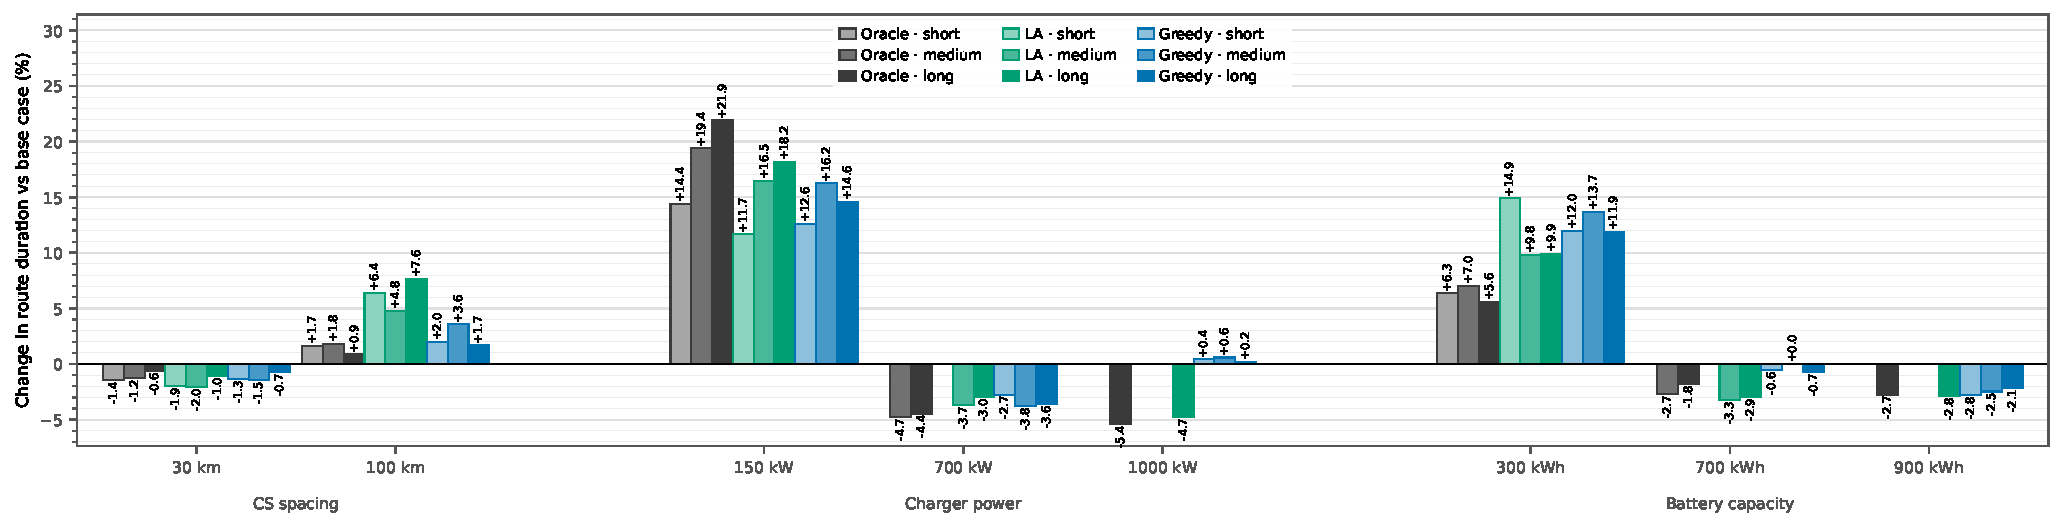
\includegraphics[width=0.8\linewidth]{figures/additional_sens_effects.pdf}
    \caption{One-at-a-time sensitivity of mean route duration to the charging
    infrastructure and uncertainty parameters, relative to the base case, over
    the 160 paired instances of Section~\ref{sec:additional-protocol}.  Axes
    without completed runs are drawn as explicit ``pending'' slots.
    \red{Regenerate once the oracle legs of the sweeps have finished; the bars
    shown are the Greedy policy.}}
    \label{fig:sens}
\end{figure}

\red{The results below are preliminary: they are the Greedy legs of the sweeps,
which are complete, whereas the oracle legs are still running.  Greedy responds
to a parameter change through both the problem and its own myopia, so the
magnitudes should be treated as upper bounds on the true problem sensitivity
until the oracle columns of Table~\ref{tab:sensitivity} are filled.}

Charger power dominates charger density, by roughly a factor of four over the
policy-relevant range.  Halving the AFIR spacing from 60 to 30\,km buys only
1.6\% of route duration, while doubling it to 90\,km costs 2.6\%: at the
mandated spacing the corridor is already dense enough that the binding
constraint is how long a charging stop takes, not how far away the next one is.
Upgrading the charger from the 200\,kW base to 350\,kW saves 9.6\%, and going
all the way to a 1\,MW megawatt-charging system saves 11.1\%---so a 350\,kW
charger already captures 86\% of the benefit available at five times the power.
Downgrading to 150\,kW, conversely, costs 9.3\%.  The asymmetry is a direct
consequence of the concave charging curve: at low power the truck spends its
time in the slow final segment, and adding power shortens exactly that segment;
once the fast segments are short relative to the mandatory rest periods, extra
power has nothing left to remove.  This is the same coupling mechanism that
Section~\ref{sec:diesel} quantifies from the other direction, and it is the
practically actionable finding of this section: for a corridor already built
out to AFIR spacing, investment should go into power per pool rather than into
more pools.

\red{Once the CV and $\beta$ sweeps land, the expected narrative is that
raising CV degrades the committing methods faster than the adaptive ones (it is
the axis on which LA's re-optimisation earns its cost) and that raising $\beta$
shifts the penalised gap composition documented in Section~\ref{sec:basecase}.
Do not write those sentences before the runs exist.}


\subsection{Comparison with diesel trucks}
\label{sec:diesel}

To separate the cost of \emph{electrification} from the cost of
\emph{scheduling}, every instance of the subset in
Section~\ref{sec:additional-protocol} is re-solved as a diesel vehicle.  Diesel
mode removes the energy dimension entirely---per-leg consumption is set to
zero, the battery starts and stays full, and the charging-station overheads
(stop, sequencing) are zeroed---while keeping the node set, the customer windows
and the full Hours-of-Service machinery intact.  Former charging stations remain
as break-eligible waypoints, so the diesel problem is a genuine relaxation of
the electric one on the same corridor and the same travel-time realisation, and
the two are solved by the same oracle and the same greedy policy.  All 160
instance pairs completed for both Greedy and the oracle.

\begin{table}[htbp]
\centering
\caption{Electric versus diesel route duration on identical instances and
realizations.  ``Naive'' adds the EV's total charging time to the diesel
makespan, i.e.\ the penalty a planner would predict who ignored that charging
can share time with a mandatory rest.  ``Coupling'' is the share of charging
time credited inside a mandatory break, $\sum_i g_i / \sum_i \tau^c_i$, at the
hindsight optimum.  $n = 80$ instances per route class.}
\label{tab:diesel}
\begin{tabular}{lrrrrrr}
\toprule
\textbf{Route} & \textbf{Diesel (h)} & \textbf{EV (h)} & \textbf{Charging (h)} & \textbf{Naive (\%)} & \textbf{Oracle (\%)} & \textbf{Coupling (\%)} \\
\midrule
Short  & 27.49 & 27.36 & 0.75 & $+2.74$ & $-0.47$ & 59 \\
Medium & 54.98 & 54.58 & 1.79 & $+3.26$ & $-0.63$ & 58 \\
\bottomrule
\end{tabular}
\end{table}

\begin{figure}[htbp]
    \centering
    % \red{PLACEHOLDER} — produced by `python additional_figures.py --section diesel`:
    % figures/additional_diesel_gap.pdf
    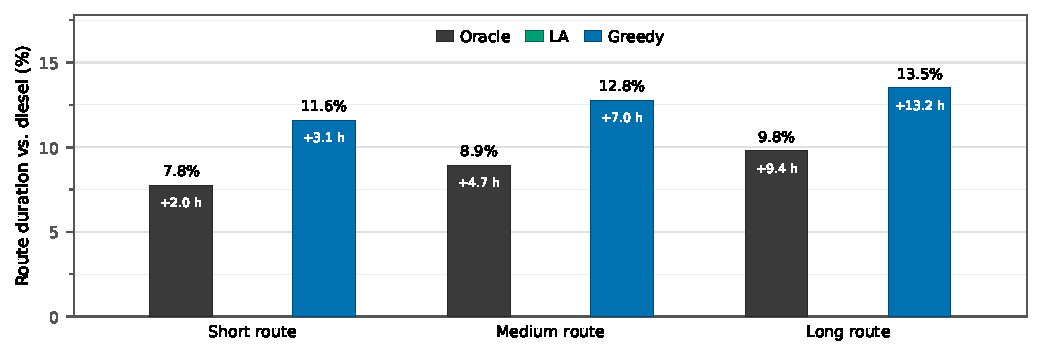
\includegraphics[width=0.75\linewidth]{figures/additional_diesel_gap.pdf}
    \caption{Electrification penalty in route duration, per route class: the
    naive estimate (diesel makespan plus the EV's total charging time) against
    the penalty actually realized by the greedy policy and by the hindsight
    optimum.  The annotation below each group gives the mean coupling share
    $\sum_i g_i/\sum_i \tau^c_i$ and the number of instances.}
    \label{fig:diesel}
\end{figure}

The headline result is that, under optimal planning, electrification is
essentially free in makespan terms on these corridors.  A planner who simply
adds the required charging time to the diesel schedule would predict a penalty
of 2.7\% on the short routes and 3.3\% on the medium ones (0.75\,h and 1.79\,h
of charging on 27\,h and 55\,h of driving).  The hindsight optimum realizes
$-0.5\%$ and $-0.6\%$: statistically indistinguishable from zero, and far below
the naive figure.  The mechanism is the coupling that motivates the model.
Across both route classes, 58--59\% of charging time is credited inside a
mandatory HoS break, and once a break must be taken anyway, plugging in during
it costs nothing in makespan.  The residual charging that cannot be hidden
inside a rest is small enough to be absorbed by re-timing the remaining breaks.

\red{Two caveats must be stated in the paper, because the sign of the oracle
column is not physically possible.}  Diesel mode is a relaxation of the
electric problem on the same instance, so a \emph{true} electric optimum can
never be shorter than the diesel one; the mildly negative means (individual
values range from $-2.3$ to $+1.4\%$ on short and $-3.7$ to $+7.2\%$ on medium
routes, with the electric schedule longer in only 28\% and 20\% of instances)
come from two sources.  First, the oracle objective is arrival time
\emph{plus} $\beta\sum_i \delta_i$, whereas Table~\ref{tab:diesel} compares
duration alone: the two worlds trade duration against window misses
differently, and a diesel optimum is free to arrive later in exchange for
hitting more windows.  Second, only 8 of 160 electric and 1 of 160 diesel
oracle solves are closed to proven optimality within the time cap; the mean
residual MIP gap is 0.5\% and reaches 10--11\% in the worst cases, which is the
same order as the effect being measured.  \red{Recommended fix before
submission: report Table~\ref{tab:diesel} on the penalised objective
(arrival $+\,\beta\sum_i\delta_i$) rather than duration alone, so both columns
are measured in the quantity the oracle actually minimises; the conclusion
``the optimal electrification penalty is an order of magnitude below the naive
estimate'' is robust either way, but the negative sign is an artefact and a
referee will catch it.}

The greedy comparison tells the complementary half of the story, and it is
where the practically important number lies.  Greedy's electric schedule is
20.7\% longer than its own diesel schedule on the short routes and 24.2\%
longer on the medium ones---an order of magnitude above the optimal penalty.
Almost none of that is electrification: measured against its own hindsight
optimum, Greedy loses 18.6\% (short) and 21.5\% (medium) on the electric
problem, and essentially nothing on the diesel problem, where the myopic rule
is already near-optimal because the only decision left is when to rest.
\red{The diesel greedy figure is in fact $-2.1\%$ and $-3.0\%$ ``better than
optimal'', for the same duration-versus-penalised-objective reason as above ---
another argument for switching the whole section to the penalised objective.}
The conclusion, stated carefully: the makespan cost of electrifying a long-haul
corridor is not a physical cost of charging but a cost of \emph{planning}
quality.  With a myopic rule it is 20--24\%; with a planner that exploits the
break/charge coupling it is close to zero.  This is the strongest argument in
the paper for the model itself, and it is the argument the sensitivity of
Section~\ref{sec:sensitivity} supports from the infrastructure side: a 350\,kW
upgrade buys 9.6\%, while better scheduling on existing 200\,kW infrastructure
buys twice that.


\subsection{Effect of uncertainty}
\label{sec:uncertainty}

The final block isolates what uncertainty itself costs, along three lines: what
it does to window compliance, how much of the loss can be recovered by adapting
en route, and how much would remain even with perfect information.

\paragraph{Uncertainty is paid in windows, not in driving time.}
This is already visible in the base case, without any additional run.  The two
gap definitions of Tables~\ref{tab:gap} and \ref{tab:gap-nopen} differ only by
the $\beta\sum_i\delta_i$ term, and their difference is concentrated exactly
where uncertainty has the most to disrupt: on the window-free classes the two
coincide to the last digit, whereas on the tight-window classes the penalty
term accounts for 25\% of RO's gap, 35\% of SP's, 37\% of Greedy's, 38\% of
LA's and 42\% of ROBU's, rising to two-thirds for Greedy on
\emph{Short}/\emph{Many}/\emph{Tight}.  Window compliance is also the axis on
which the methods separate most: 44.9\% (RO), 55.0\% (Greedy), 67.3\% (ROBU),
69.7\% (LA), 86.6\% (SP) in Table~\ref{tab:feasibility}, against a spread of
only a few percentage points in HoS violations.  A schedule committed before
departure survives the travel-time noise in its rest structure and fails in its
appointments.

\paragraph{Adapting en route recovers most of the loss.}
The same table quantifies the price of that adaptation.  SP reaches its 86.6\%
window hit rate by repairing its committed structure on 99.0\% of executions,
and pays for it with an 11.6\% stranding rate; LA reaches 69.7\% with no
recourse machinery at all but 14--23\,s of re-optimisation per stop and a 1.0\%
stranding rate.  The comparison across route classes in Table~\ref{tab:gap}
sharpens this: full re-optimisation at every stop (LA) degrades gracefully with
route length (12.3\%, 13.8\%, 10.6\% mean gap), whereas a scenario set fixed at
departure (SP) is excellent on short routes (5.5\%), no better than LA on
medium ones (13.8\%), and unusable on long ones.  The value of re-planning is
therefore not uniform---it grows with the horizon over which the initial
scenario set becomes stale.

\paragraph{Price of robustness.}
The budgeted robust model interpolates between the nominal plan
($\Gamma = 0$) and the box $(\Gamma = N$, i.e.\ RO), and the base case fixes
$\Gamma = \sqrt{N}$.  Figure~\ref{fig:gamma} traces the whole frontier on the
short routes: realized gap to oracle above, realized infeasibility below, so
the conservatism/reliability trade-off can be read directly rather than
inferred from two endpoints.  \red{Only the endpoints exist so far
($\Gamma = \sqrt{N}$: 23.7\% gap; $\Gamma = N$: 32.7\% gap, both averaged over
the twelve short-route classes).  The sweep is launched with
\texttt{python additional\_analysis.py gamma -{}-gammas 0,1,2,4,8
-{}-combos RshortCfew,RshortCmany}.  This is also the experiment that should
explain ROBU's 3.3\% stranding rate: if strandings grow as $\Gamma$ falls, the
cause is the budget; if they are flat in $\Gamma$, the cause is the energy
corner and not the time budget.}

\begin{figure}[htbp]
    \centering
    % \red{PLACEHOLDER} — produced by `python additional_figures.py --section gamma`:
    % figures/additional_gamma_frontier.pdf
    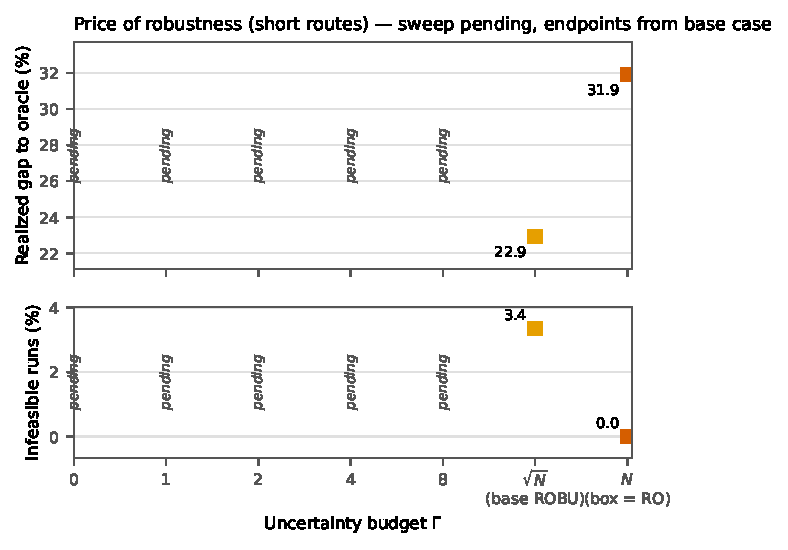
\includegraphics[width=0.7\linewidth]{figures/additional_gamma_frontier.pdf}
    \caption{Price of robustness on the short routes: realized gap to the
    oracle (top) and realized infeasibility rate (bottom) as a function of the
    uncertainty budget $\Gamma$, from the nominal plan ($\Gamma = 0$) to the
    box ($\Gamma = N$, which coincides with RO).  \red{Interior points pending;
    the figure currently shows the two endpoints taken from the base case.}}
    \label{fig:gamma}
\end{figure}

\paragraph{Value of the stochastic solution and of perfect information.}
Finally we decompose the total cost of uncertainty on a common set of
scenarios, drawn once per instance with common random numbers so that all three
legs see identical realisations.  Let WS be the mean perfect-hindsight optimum
over the scenario set (wait-and-see); RP the mean realized objective of the
two-stage plan executed with online duration recourse; and EEV the mean
realized objective of the plan obtained from the expected-value problem---the
deterministic model solved at nominal travel times---executed under the same
recourse semantics.  Then
\begin{equation}
\mathrm{VSS} = \mathrm{EEV} - \mathrm{RP}, \qquad
\mathrm{EVPI} = \mathrm{RP} - \mathrm{WS},
\end{equation}
where VSS measures what modelling the travel-time distribution at plan time is
worth relative to planning on the mean, and EVPI the irreducible loss that no
amount of distributional modelling can recover.  Both are reported on the raw
arrival time and on the penalised objective, matching the two gap definitions
used throughout.  Because the two-stage plan is taken from the base-case SP
runs, its scenarios are not the common-random ones and the RP leg is
consequently a slight over-estimate; this is flagged in the table note.

\begin{table}[htbp]
\centering
\caption{Value of the stochastic solution (VSS) and expected value of perfect
information (EVPI), over common-random scenarios, by instance class.
$\mathrm{VSS} = \mathrm{EEV} - \mathrm{RP}$ and
$\mathrm{EVPI} = \mathrm{RP} - \mathrm{WS}$, in hours of route duration.}
\label{tab:vss}
\begin{tabular}{lrrrrrr}
\toprule
\textbf{Class} & \textbf{WS (h)} & \textbf{RP (h)} & \textbf{EEV (h)} & \textbf{VSS (h)} & \textbf{EVPI (h)} & \textbf{n} \\
\midrule
RshortCfew   & \red{--} & \red{--} & \red{--} & \red{--} & \red{--} & \red{--} \\
RshortCmany  & \red{--} & \red{--} & \red{--} & \red{--} & \red{--} & \red{--} \\
RmediumCfew  & \red{--} & \red{--} & \red{--} & \red{--} & \red{--} & \red{--} \\
RmediumCmany & \red{--} & \red{--} & \red{--} & \red{--} & \red{--} & \red{--} \\
\bottomrule
\end{tabular}
\end{table}

\red{Table~\ref{tab:vss} is a skeleton: the harness
(\texttt{experiments/vss\_evpi.py}) is implemented and wired into
\texttt{additional\_analysis.py vss}, but no instance has been run yet.  Each
instance costs $1 + n_{\text{scen}}$ oracle solves (one expected-value solve
plus one wait-and-see solve per scenario), so at 20 scenarios the four classes
above are the practical limit.  Run with
\texttt{python additional\_analysis.py vss -{}-n-scenarios 20}, then
\texttt{python additional\_figures.py -{}-section vss}.}
